\part{Training}

\section{Memory \label{sec_memory_training}}

In this section we summarize the train-time memory costs of Transformers under various training
strategies\footnote{A nice related blog post is \href{https://blog.eleuther.ai/transformer-math/}{here}. \label{foot_eleuther_math_101} }.

The memory cost is much more than simply the cost of the model
parameters. Significant factors include:
\begin{itemize}
	\item Optimizer states, like those of \pyinline{Adam}
	\item Mixed precision training costs, due to keeping multiple model copies.
	\item Gradients
	\item Activation memory\footnote{Activations refers to any intermediate value which needs to be
		      cached in order to compute backpropagation. We will be conservative and assume that the inputs
		      of all operations need to be stored, though in practice gradient checkpointing and recomputation
		      allow one to trade caching for redundant compute. In particular, flash attention
		      \cite{dao2022flashattention} makes use of this strategy.} , needed for backpropagation.
\end{itemize}
Because the activation counting is a little more involved, it is in its own section.


\begin{nicebox}{Essentials}
	Memory costs count the elements of all tensors in some fashion, both from model parameters and
	intermediate representations. The gradient and optimizer state costs scale with the former quantity:
	$ \Ocal \left ( N _{ {\rm params}  } \right ) \sim \Ocal \left ( L D ^{ 2 } \right )$, only counting
	the dominant contributions from weight matrices. Activation memory scales with the latter,
	which for a \pyinline{(B, S, D)}-shaped input gives $ \Ocal \left ( BDLS  \right ) $ contributions
	from tensors which preserve the input shape, as well as $ \Ocal \left( ABLS ^{ 2 } \right)  $
	factors from attention matrices.
\end{nicebox}


\subsection{No Sharding}

Start with the simplest case where there is no sharding of the model states. Handling the different
parallelism strategies later will be relatively straightforward, as it involves inserting just a few
factors here and there.

\subsubsection{Parameters, Gradients, Optimizer States, and Mixed Precision
	\label{sec_params_grads_optim_mem}}


Memory from the bare parameter cost, gradients, and optimizer states are fixed costs independent of
batch size and sequence-length (unlike activation memory), so we discuss them all together here. The
parameter and optimizer costs are also sensitive to whether or not mixed-precision is used, hence we
also address that topic, briefly.  We will assume the use of \pyinline{Adam}\footnote{Which stores
	\href{https://pytorch.org/docs/stable/generated/torch.optim.Adam.html}{two different running
		averages} per-model parameter.} throughout, for simplicity and concreteness. It will sometimes be
useful below to let $ p $ to denote the precision in bytes that any given element is stored in, so
\pyinline{torch.float32} corresponds to $ p=4 $, for instance. Ultimately, we primarily consider
vanilla training in $ p=4 $ precision and \pyinline{torch.float32}/\pyinline{torch.float16} ($ p=4
$/ $ p=2 $)  mixed-precision, other, increasingly popular variants to exist, so we keep the
precision variable where we can.


Without mixed precision, the total cost of the
\pyinline{torch.float32} ($ p=4 $ bytes) model and optimizer states in bytes is then
\begin{align}
	M _{ \rm model} & = 4 N _{ \rm params } \ , \quad M_{ \rm  optim } = 8 N _{ \rm params }
	\quad ({\rm no \ mixed \ precision, } p=4)
	\label{eq_optimizer_states_mem_no_mp}
\end{align}
where, from the previous section, the pure parameter-count of the decoder-only Transformers
architecture is
\begin{align}
	N _{ \rm params } & \approx  (4 + 2E) L D ^{ 2 } \times \left ( 1 + \Ocal \left( \frac{ V }{ DL }
		\right) + \Ocal \left( \frac{ 1 }{ D } \right)  \right ) \ . \label{eq_approx_params_no_sharding}
\end{align}
where the first term comes from the \pyinline{TransformerBlock} weight matrices\footnote{So,
	in the usual $ E=4 $ case, the \pyinline{MLP} layers are twice as costly as the
	\pyinline{CausalAttention} layers.}, the first omitted subleading correction term is the embedding
matrix, and the last comes from biases, \pyinline{LayerNorm} instances, and other negligible
factors.  The optimizer states cost double the model itself.


The situation is more complicated when mixed-precision is used \cite{micikevicius2018mixed}.
The pertinent components of mixed-precision\footnote{A note on the implementation of mixed-precision
in \pyinline{torch}: usually mixed-precision occurs by wrapping the forward pass in a context
manager, \pyinline{torch.autocast}. The default behavior is to then create copies of some tensors
in lower-precision and do the forward pass with those. For instance, this is done with
matrix-multiplies whose arguments and outputs will be in \pyinline{torch.float16}, but for sums
the inputs and outputs will all be \pyinline{torch.float32}, for vanilla mixed-precision usage.
Consequently, any such \pyinline{torch.float16} versions of tensor will often persist effectively
as contributors to activation memory, since the backwards pass will need those same tensors. This
can be verified by inspecting the saved tensors: if \pyinline{z} is the output of a
matrix-multiply in such an autocast context, \pyinline{z.grad_fn._saved_mat2} will be a
\pyinline{torch.float16} copy of the weights used to perform the matrix-multiply. In effect, the
cost of the model weights which are used for the actual forward pass are only materialized within
the lifetime of the context manager.}:
\begin{itemize}
	\item A half-precision ($ p=2 $ bytes) copy of the model is used to perform the forwards and
	      backwards passes
	\item A second, "master copy" of the model is also kept with weights in full $ p=4 $ precision
	\item The internal \pyinline{Adam} states are kept in full-precision
\end{itemize}
Confusingly, the master copy weights are usually accounted for as part of the optimizer state, in
which case the above is altered to
\begin{align}
	M _{ \rm model} & = 2 N _{ \rm params } \ , \quad M_{ \rm  optim } = 12 N _{ \rm params }
	\quad ({\rm mixed \ precision}) .
	\label{eq_optimizer_states_mem_mp}
\end{align}
The optimizer state is now six times the cost of the actual model used to process data and the costs
of \eqref{eq_optimizer_states_mem_mp} are more than those of \eqref{eq_optimizer_states_mem_no_mp}.
However, as we will see, the reduced cost of activation memory can offset these increased costs, and
we get the added benefit of increased speed due to specialized hardware. The above also demonstrates
why training is so much more expensive than inference.


\subsubsection{Gradients}

Gradients are pretty simple and always cost the same regardless of whether or not mixed-precision is
used:
\begin{align}
	M_{ \rm grad} & = 4 N _{ \rm params }     \label{eq_grad_memory} \ .
\end{align}
In mixed precision, even though the gradients are initially computed in $ p= 2$, they
\href{https://huggingface.co/docs/transformers/v4.20.1/en/perf_train_gpu_one#anatomy-of-models-memory}{have to
	be converted} to $ p=4 $ to be applied to the master weights of the same precision.




\subsubsection{Activations}

Activations will require a more extended analysis \cite{korthikanti2022reducing}. Unlike the above
results, the activation memory will depend on both the batch size and input sequence length, $ B $
and $ S $, scaling linearly with both.



\paragraph{Attention Activations}

We will count the number of input elements which need to be cached. Our \pyinline{(B, S, D)}-shaped inputs
to the attention layer with $ BDS $ elements are first converted to $ 3BDS $ total query, key, value
elements, and the query-key dot products produce $ ABS ^{ 2 } $ more, which are softmaxed into $ ABS
		^{ 2 } $ normalized scores. The re-weighted inputs to the final linear layer also have $ BDS $
elements, bringing the running sum to $ BS \left ( 5D + 2AS  \right ) $

Finally, there are also the dropout layers applied to the normalized attention scores and the final
output whose masks must be cached in order to
backpropagate. In torch, the mask is a \pyinline{torch.bool} tensor, but
\href{https://github.com/pytorch/pytorch/issues/41571}{surprisingly} these use one \textit{byte} of
memory per element, rather than one bit \footnote{As you can verify
	via \pyinline{4 * torch.tensor([True]).element_size() == torch.tensor([1.]).element_size().}}.
Given this, the total memory cost from activations is
\begin{align}
	M _{ \rm act  } ^\texttt{Attention} & = BLS \left ( (5p+1)D + (2p+1)AS  \right ) \ .
	\label{eq_att_actmem_vanilla}
\end{align}




\paragraph{MLP Activations}

First we pass the \pyinline{(B, S, D)}-shaped inputs into the first MLP layer. These turn into the
\pyinline{(B, S, E*D)} inputs of the non-linearity, whose same-shaped outputs are then passed into
the last \pyinline{Linear} layer, summing to $ (2E+1)BDS $ total elements thus far. Adding in the
dropout mask, the total memory requirement across all \pyinline{MLP} layers is:
\begin{align}
	M _{ \rm act  } ^\texttt{MLP} & = (2Ep+p+1)BDLS\ .
	\label{eq_mlp_actmem_vanilla}
\end{align}




\paragraph{LayerNorm, Residual Connections, and Other Contributions}

Then the last remaining components. The \pyinline{LayerNorm} instances each have $ BDS $ inputs and
there are two per transformer block, so $ M _{ {\rm  act}  } ^\texttt{LayerNorm} = 2pBDLS $, and
there is an additional instance at the end of the architecture\footnote{Following
\cite{korthikanti2022reducing} we will neglect this in the below sum, an $ \Ocal \left( 1/L
\right) $ error}. There are two residual connections per block, but their inputs do not require
caching (since their derivatives are independent of inputs). Then, there are additional
contributions from pushing the last layer's outputs through the language-model head and
computing the loss function, but these do not scale with $ L $ and are ultimately $ \sim \Ocal
\left( \frac{ V }{ DL } \right)  $ suppressed, so we neglect them.





\paragraph{Total Activation Memory}


Summing up the contributions above, the total activation memory cost per-layer is
\begin{align}
	M _{ {\rm act}  } ^{ {\rm  total}  } & \approx  2BDLS   \left ( p(E+4) + 1 + \Ocal \left( \frac{
		V}{ DL } \right)  \right )
	+ ABLS ^{ 2 } \left ( 2p+1\right ) \label{eq_act_mem_total_no_sharding}\ .
\end{align}
Evaluating in common limits, we have:
\begin{align}
	M _{ {\rm act}  } ^{ {\rm  total}  } \Big| _{ E=4, p=4 } & =BLS \left ( 66 D+15AS  \right ) \nn
	M _{ {\rm act}  } ^{ {\rm  total}  } \Big| _{ E=4, p=2 } & =BLS \left ( 34 D+5AS  \right )
\end{align}


\paragraph{When does mixed-precision reduce memory?} (Answer: usually.) We saw in Sec.~\ref{sec_params_grads_optim_mem}
that mixed precision \textit{increases} the fixed costs of non-activation memory, but from the above
we also see that it also \textit{reduces} the activation memory and the saving increase with larger
batch sizes and sequence lengths. It is straightforward to find where the tipping point is.
Specializing to the case $E=4$, vanilla mixed-precision case with no parallelism\footnote{With both
	tensor- and sequence-parallelism, the parallelism degree $ T $ actually drops out in the comparison
	(since both form of memory are decrease by $ 1/T $, so this restriction  can be lifted.}, the
minimum batch size which leads to memory savings is
\begin{align}
	B _{ {\rm min}  } & = \frac{ 6 D ^{ 2 } }{ 8 DS + A S ^{ 2 } }\label{eq_min_mp_batch_size}\ .
\end{align}
Plugging in numbers for the typical $ \Ocal \left( 40 \ {\rm GiB} \right)$ model in the Summer of
2023 gives $ B _{ {\rm min} } \sim \Ocal \left( 1\right)  $, so mixed-precision is indeed an overall
savings at such typical scales.



\begin{commentbox}{Side Note: Optimizations}

The above analysis is conservative and accounts for more tensors than are actually saved in
practice.\newline

For instance, both the input and outputs of all non-linearities were counted, but there are many
activations whose derivatives can be reconstructed from its outputs alone: $ \phi'(z)=F \left (
\phi(z) \right ) $ for some $ F $. Examples:
\begin{itemize}
    \item \pyinline{ReLU}: since $ \phi(z)= z\theta(z) $, then (defining the derivative at zero to
        be zero) $ \phi'(z) =\theta(z) = \theta \left ( \phi(z) \right) $. Correspondingly, torch
        only uses the \pyinline{ReLU} outputs \href{https://github.com/pytorch/pytorch/blob/73d288fdf9d0beb76229cabc8566ee116f8a21a2/tools/autograd/derivatives.yaml#L2009-L2011}{to compute the derivative}
        (there is no self arg in the \pyinline{threshold_backward(grad, result, 0)} line).
    \item  \pyinline{tanh}: since $ \tanh'(z)=1-\tanh(z) ^{ 2 } $.
\end{itemize}
Other cases do not have this nice property, in which case both the inputs and outputs need to
be stored:
\begin{itemize}
    \item \pyinline{GeLU} \cite{hendrycks2023gaussian}: $ \phi(z)=z\Phi(z) $ here and the derivative
        $ \phi'(z)= \Phi(z) + \frac{ z e^{ -z ^{ 2 } /2 } }{\sqrt{2\pi}  } $, both the inputs and
        outputs \href{https://github.com/pytorch/pytorch/blob/73d288fdf9d0beb76229cabc8566ee116f8a21a2/tools/autograd/derivatives.yaml#L2041-L2044}{must be used in the backwards pass.}.

        The explicit CUDA kernel \href{https://github.com/pytorch/pytorch/blob/73d288fdf9d0beb76229cabc8566ee116f8a21a2/aten/src/ATen/native/cuda/ActivationGeluKernel.cu#L70-L84}{is here}.
\end{itemize}
If the inputs in each of these cases are not needed for any other part of the backwards pass, they
are garbage collected in \pyinline{torch} soon after creation.


\paragraph{Example}: \pyinline{Softmax} is another instance where this occurs, since
\begin{align}
     \partial _{ i } \Sm \left ( x _{ j } \right )  &= \delta _{ ij }\Sm \left ( x _{ j } \right ) -   \Sm \left ( x _{ i } \right )  \Sm \left ( x _{ j } \right ) \label{eq_softmax_derivative}
\end{align}
Because of this, the actual amount of activation memory due to the attention layer after the
forwards pass is \eqref{eq_att_actmem_vanilla} with $ 2p \longrightarrow p $ in the $ \Ocal \left( S
^{ 2 } \right)  $ term, though the above expression better reflects the necessary peak memory.

\end{commentbox}


\subsection{Case Study: Mixed-Precision GPT3 \label{subsec_gpt_mem_study} }

Let's run through the numbers for mixed-precision GPT3 with
\href{https://bmk.sh/2020/05/29/GPT-3-A-Brief-Summary/}{parameters}:
\begin{align}
	L & = 96 \ , \quad
	D = 12288 \ ,\quad
	A = 96\ , \quad V = 50257\ .
	\label{eq_gpt_num}
\end{align}
We are leaving the sequence-length unspecified, but the block-size (maximum sequence-length) is $
	K=2048 $.


Start by assuming no parallelism at all. The total (not per-layer!) non-activation memory is
\begin{align}
	M _{ {\rm non-act}  } ^ \texttt{GPT-3} & \approx 1463\ {\rm TiB}
\end{align}
which can be broken down further as
\begin{align}
	M _{ {\rm params}  } ^ \texttt{GPT-3} & \approx 162\ {\rm TiB} \ , \quad
	M _{ {\rm grads}  } ^ \texttt{GPT-3}  \approx 325\ {\rm TiB}\ , \quad
	M _{ {\rm optim}  } ^ \texttt{GPT-3}  \approx 975\ {\rm TiB}\ .
\end{align}
The embedding matrix only makes up $ \approx .3\% $ of the total number of parameters, justifying our
neglect of its contribution in preceding expressions.


The activation memory is
\begin{align}
	M _{ {\rm act}  } ^ \texttt{GPT-3} & \approx 3 \times 10 ^{ -2 }BS\times  \left (  1  + \frac{ S
	}{ 10 ^{ 3 } } \right ) \ {\rm TiB} \ .
\end{align}
Note that the attention matrices, which are responsible for $ \Ocal \left( S ^{ 2 } \right)  $ term, will
provide the dominant contribution to activation memory in the usual $ S \gtrsim 10 ^{ 3 } $ regime.

In the limit where we process the max block size ($ S=K=2048 $), the ratio of activation to
non-activation memory is
\begin{align}
	\frac{  M _{ {\rm act}  } ^ \texttt{GPT-3}}{ M _{ {\rm non-act}  } ^ \texttt{GPT-3} }\Big| _{
	S=2048 } & \approx  .2 B \ .
\end{align}
So, the activation memory is very significant for such models.


Using tensor parallelism into the above with the maximal $ T=8 $ which can be practically used, the
savings are significant. The total memory is now
\begin{align}
	M _{ {\rm total}  } ^{ \texttt{GPT-3}  } & \approx 187\ {\rm TiB} + 10 ^{ -2 }BS + 5 \times 10 ^{
			-6} BS ^{ 2 }\ .
\end{align}




\section{Training FLOPs \label{sec_flops_training} }

The total number of floating point operations (FLOPs)\footnote{The notation surrounding
	floating-point operations is very confusing because another quantity of interest is the number
	of floating-point operations a given implementation can use \textit{per-second}. Sometimes,
	people use FLOPS or FLOP/s to indicate the rate, rather than the gross-count which has the lower
	case ``s", FLOPs, but there's little consistency in general. We will use FLOPs and FLOP/s.}  needed to process a given batch of
data is effectively determined by the number of matrix multiplies needed.

Recall that a dot-product of the form $ v \cdot M $  with $ v \in \mathbb{R}^{ m } $ and $ M \in
	\mathbb{R} ^{ m, n }$ requires $ \left (2 m-1 \right )\times n \approx 2mn$ FLOPs .
For large language models, $ m,n \sim \Ocal \left( 10 ^{ 3 } \right)  $, meaning that even expensive
element-wise operations like \pyinline{GeLU} acting on the same vector $ v $ pale in comparison by
FLOPs count \footnote{Since their FLOPs counts only scales as $ \sim \Ocal \left( n\right )  $ where
	the omitted constant may be relatively large, but still negligible when all dimensions are big.}. It
is then a straightforward exercise in counting to estimate the FLOPs for a given architecture. The
input tensor is of shape \pyinline{(B, S, D)} throughout.

\begin{nicebox}{Essentials}
	The number of FLOPs to push a batch of $ B $ of sequence-length $ S $ examples through the forwards-pass
	of a decoder-only transformer is approximately $ 2BS N _{ {\rm params}  } $ where the number of
	parameters accounts for any reductions due to tensor- and sequence-parallelism\footnote{A quick argument: a
	computation of the form $T _{ a _{ 0 }\ldots  a _{ n }j } =V _{ a _{ 0 }\ldots a _{ A
			}i }M _{ ij } $ requires $ 2A _{ 0 }\ldots A _{ n }IJ $ FLOPs where the capital letters
	represent the size of their similarly-index dimensions. Thus, the FLOPs
	essentially count the size of the matrix $ M $ (that is, $ IJ $), up to a factor of 2 times all of the
	dimensions in $ V $ which weren't summed over. Therefore, passing a
	\pyinline{(B, S, D)}-shaped tensor through the Transformer architecture would give $ \sim 2BS\times
	$(sum of sizes of all weight-matrices) FLOPs, and that this last factor is also approximately the number of
	parameters in the model (since that count is dominated by weights). Thus, FLOPs $ \approx 2BSN _{
				{\rm params}  } $. This is the correct as long as the self-attention FLOPs with $ \Ocal \left( S ^{ 2 } \right)$-dependence which we
	didn't account for here are actually negligible (true for $ S \lesssim 10  D $).}. The backwards-pass
	costs about twice as much as the forwards-pass. This is true as long as $ S \lesssim D $).
\end{nicebox}



\subsection{No Recomputation}

Start with the case where there is no recomputation activations.  These are the \textbf{model FLOPs} of
\cite{korthikanti2022reducing}, as compared to the \textbf{hardware FLOPs} which account for gradient
checkpointing.


\paragraph{\pyinline{CausalAttention}: Forwards }

The FLOPs costs:
\begin{itemize}
	\item  Generating the query, key, and value vectors: $ 6BSD ^{ 2 } $
	\item Attention scores:  $2BDS ^{ 2 }$
	\item Re-weighting values:  $2BDS ^{ 2 }$
	\item Final projection: $ 2BSD ^{ 2 } $
\end{itemize}

\paragraph{\pyinline{MLP}: Forwards}
Passing a  through the \pyinline{MLP} layer, the FLOPs due to the
first and second matrix-multiplies are equal, with total matrix-multiply FLOPs  $ 4BSED ^{ 2 } $.

\paragraph{Backwards Pass: Approximate}


The usual rule of thumb is to estimate the backwards pass as costing twice the flops as the forwards
pass. This estimate comes from just counting the number of $ \Ocal \left( n ^{ 2 } \right)$
matrix-multiply-like operations and seeing that for every one matrix multiplication that was needed
in the forward pass, we have roughly twice as many similar operations in the backwards pass.


The argument: consider a typical sub-computation in a neural network which is of the form $ z' =
	\phi \left ( W \cdot z \right ) $ where $ z', a $ are intermediate representations $ z, z' $, $ \phi
$ is some non-linearity, and where the matrix multiply inside the activation function dominates the
forwards-pass FLOPs count, as above.  Then, in the backwards pass for this sub-computation, imagine
we are handed the upstream derivative $ \partial _{ z '  } \Lcal $. In order to complete
backpropagation, we need both to compute $ \partial  _{ W }\Lcal  $ to update $ W $ and also $
	\partial  _{ z } \Lcal  $ to continue backpropagation to the next layer down. Each of these operations
will cost about as many FLOPs as the forwards-pass, hence the estimated factor of two (but, as
we will see, this is a very rough estimate).

Being more precise, let $ z $ be \pyinline{(D0, ... , Dn, J)}-shaped and let $ W $ be
\pyinline{(I, J)}-shaped such that it acts on the last index of $ z $, making $ z' $
\pyinline{(D0, ... , Dn, I)}-shaped. Denoting $D=\prod _{ i } D _{ i } $ be the number of elements
along the $ D _{ i } $ directions for brevity, the forward-FLOPs cost of the sub-computation is
therefore $ 2DIJ$.


Adding indices, the two derivatives we need are
\begin{align}
    \frac{ \partial \Lcal  }{ \partial W _{ ij } } & = \frac{ \partial \Lcal  }{ \partial z '_{ d _{ 0 } \ldots  d _{ n }i } }\phi' \left (\left (  W \cdot z \right ) _{  d _{ 0 }\ldots d _{ n }i } \right )
	z _{ d _{ 0 }\ldots  d _{ n } j } \nn
	\frac{  \partial \Lcal  }{\partial  z _{ d _{ 0 }\ldots d _{ n }j } } & = \frac{ \partial \Lcal
	}{ \partial z '_{ d _{ 0 } \ldots  d _{ n }i } }\phi' \left (\left (  W \cdot z \right ) _{  d _{
			0 }\ldots d _{ n }i } \right ) W _{ ij }\ ,\label{eq_backprop_derivatives}
\end{align}
which have shapes \pyinline{(I, J)} and \pyinline{(D0, ..., Dn, J)}, respectively. On the right
side, $ z $ and $ W \cdot  z $ are cached and the element-wise computation of $ \phi' \left ( W
\cdot z \right ) $ has negligible FLOPs count, as discussed above: its contribution is $ \Ocal
\left( 1/I \right)  $ suppressed relative to the matrix-multiplies. The FLOPs count is instead
dominated by the broadcast-multiplies, sums, and matrix-products.

The two derivatives in \eqref{eq_backprop_derivatives} each have the same first two factors in
common, and it takes $ DI $ FLOPs to multiply out these two \pyinline{(D0, ... , Dn, J)}-shaped
tensors into another result with the same shape. This contribution is again $ \Ocal \left( 1/I
\right)  $ suppressed and hence negligible. Multiplying this factor with either $ z
_{ d _{ 0 } \ldots d _{ n }i } $ or $ W _{ ij } $ and summing over the appropriate indices requires
$ 2DIJ $ FLOPs for either operation, bringing the total FLOPs to $ 4DIJ$, which is double the FLOPs
for this same sub-computation in the forward-direction, hence the rough rule of thumb\footnote{Note
    also that the very first layer does not need to perform the second term in
    \eqref{eq_backprop_derivatives}, since we do not need to backpropagate to the inputs, so the
    total backwards flops is more precisely $ 4DIJ(L-1) + 2DIJ$.}.


\paragraph{Backwards Pass: More Precise} \textbf{TODO}

\paragraph{Total Model FLOPs}


The grand sum is then\footnote{With a large vocabulary, the cost of the final language model head
	matrix multiply can also be significant, but we have omitted its $ L $-independent,  $ 2BDSV $
	contribution here. }:
\begin{align}
	C  ^{ {\rm  model}  } & \approx 12 BDLS \left ( S + \left ( 2+E \right )D \right ) \label{eq_model_flops}\ .
\end{align}
We can also phrase the FLOPs in terms of the number of parameters \eqref{eq_approx_params_tensor_parallel} as
\begin{align}
	C  ^{ {\rm  model}  } \big| _{ T=1 } & = 6BS N _{ {\rm  params}  }\times \left ( 1 + \Ocal \left( S/D\right)  \right )
\end{align}
where we took the $ T=1, D \gg S $ limit for simplicity and we note that $ BS $  is the number of
total tokens in the processed batches.


\section{Training Time \label{sec_train_time} }



Training is generally compute bound (see App.~\ref{app_compute_mem_bound}) and based on the results
of Sec.~\ref{sec_flops_training} the quickest one could possibly push a batch of data through the
model is
\begin{align}
	t _{ {\rm  min} } & = \frac{ C  ^{ {\rm  model}  }  }{   \lambda _{ {\rm FLOP/s} } }\ . \label{eq_tmin_model}
\end{align}
Expanding to the entire training run, then with perfect utilization training will take a time
\begin{align}
	t _{ {\rm  total} } & \approx  \frac{6N _{ {\rm params} } N _{ {\rm tokens} }}{   \lambda _{ {\rm FLOP/s} } }\ . \label{eq_training_rule_of_thumb}
\end{align}
Adjust $ \lambda _{ {\rm FLOP/s} } $ to the actual achievable FLOP/s in your setup to get a realistic estimate.

How many tokens should a model of size $ N _{ {\rm params} } $? Scaling laws (Sec.~\ref{sec_scaling_laws}) provide
the best known answer, and the Summer 2023 best-guess is that we optimally have $ N _{ {\rm tokens} }\approx 20 N _{ {\rm params} } $.
So that the above is
\begin{align}
	t _{ {\rm  total} } & \approx  \frac{120N _{ {\rm params} } ^{ 2 }}{   \lambda _{ {\rm FLOP/s} } }\ ,
\end{align}
leading to quadratic growth in training time.


Note that the above is only correct if we are actually only spending $C  ^{ {\rm  model}  }$
compute per iteration. This is not correct if we use gradient checkpointing and recomputation, in which case
we alternatively spend true compute  $C  ^{ {\rm  hardware}  } > C  ^{ {\rm  model}  } $,
a distinction between \textbf{hardware FLOPs} and \textbf{model FLOPs}. Two corresponding efficiency
measures are \textbf{model FLOPs utilization} (MFU) and \textbf{hardware FLOPs utilization}  (HFU).
If our iterations take actual time $ t _{ {\rm iter} } $, then these are given by
\begin{align}
	{\rm MFU} & = \frac{ t _{ {\rm iter} } }{ t _{ {\rm  min} } ^{ {\rm  model} } } \ , \quad {\rm HFU} = \frac{ t _{ {\rm iter} } }{ t _{ {\rm  min} } ^{ {\rm  hardware} } } \ , \label{eq_mfu}
\end{align}
where $ t _{ {\rm min} } ^{ {\rm  model} } $ is \eqref{eq_tmin_model} and $ t _{ {\rm min} } ^{ {\rm  hardware} } $ is similar but using
$ C  ^{ {\rm  hardware} } $.


\section{Scaling Laws \label{sec_scaling_laws}}


Empirically-discovered scaling laws have driven the race towards larger and larger models.
\begin{nicebox}{Essentials}
	Decoder-only model performance improves predictably as a function of the model size, dataset size,
	and the total amount of compute. As of Summer 2023, there is little sign of hitting any kind of wall
	with respect to such scaling improvements.
\end{nicebox}


The central parameters are:
\begin{itemize}
	\item The number of non-embedding model parameters, as excising embedding params was found to
	      generate cleaner scaling laws. Because our $ N _{ {\rm params} }$ has already been typically
	      neglecting these parameters, we will just use this symbol in scaling laws and keep the above
	      understanding implicit.\footnote{Presumably, the scaling laws are
		      cleaner with these neglected because these params do not contribute directly to
		      FLOPs, unlike most other parameters.} \cite{kaplan2020scaling}.
	\item $ C $: total compute, often in units like PFLOP/s-days $ \sim 10 ^{ 20 } $ FLOPs
	\item $ N _{ {\rm tokens} } $: dataset-size in tokens
	\item $\Lcal$: cross-entropy loss in nats
\end{itemize}
The specific form of any given scaling law should also be understood to apply to a pretty narrowly
defined training procedure, in which choices like the optimizer, learning-rate scheduler,
hyperparameter search budget, vocabulary size, tokenization, etc. are often rigidly set. Changing
different components of the training procedure is liable to create different scaling laws (though
nice laws of some form are still expected to exist).


\subsection{Original Scaling Laws}


The first scaling-laws were reported in \cite{kaplan2020scaling}.   Their simplest form relates the
value of the cross-entropy loss \textit{at convergence} (and in nats), $ \Lcal  $,  to the number of non-embedding
parameter, dataset size in token, and the amount of compute, \textit{in the limit} where only one of
this factors is bottlenecking the model\footnote{Unclear to me how you know when this is the case?}. The laws (in our notation):
\begin{itemize}
	\item $ \Lcal (N _{ {\rm params} }) \approx  \left ( N _{ {\rm  params} }^{ \star } / N _{ {\rm  params}
		      } \right ) ^{ \alpha _{ N } } $, with $ \alpha _{ N } \approx 0.076 $ and $ N _{ {\rm params} } ^{ \star }  \approx
		      8.8\times 10 ^{ 13 }$
	\item $ \Lcal (N _{ {\rm  tokens} }) \approx  \left ( N _{ {\rm tokens}} ^{ \star } / N _{ {\rm  tokens}
		      } \right ) ^{ \alpha _{ T } } $, with $ \alpha _{ T } \approx 0.095 $ and $ N _{{\rm  tokens}  } ^{  \star }  \approx
		      5.4\times 10 ^{ 13 }$
	\item $ \Lcal (C) \approx  \left ( C ^{ \star } /  C
		      \right ) ^{ \alpha _{ C } } $, with $ \alpha _{ C } \approx 0.050  $ and $ C ^{  \star }  \approx
		      3.1\times 10 ^{8} $ PFLOP/s-days, where the batch size was assumed to be chosen to be compute optimal per the criteria they outline
\end{itemize}

\begin{figure}[ht]
	\centering
	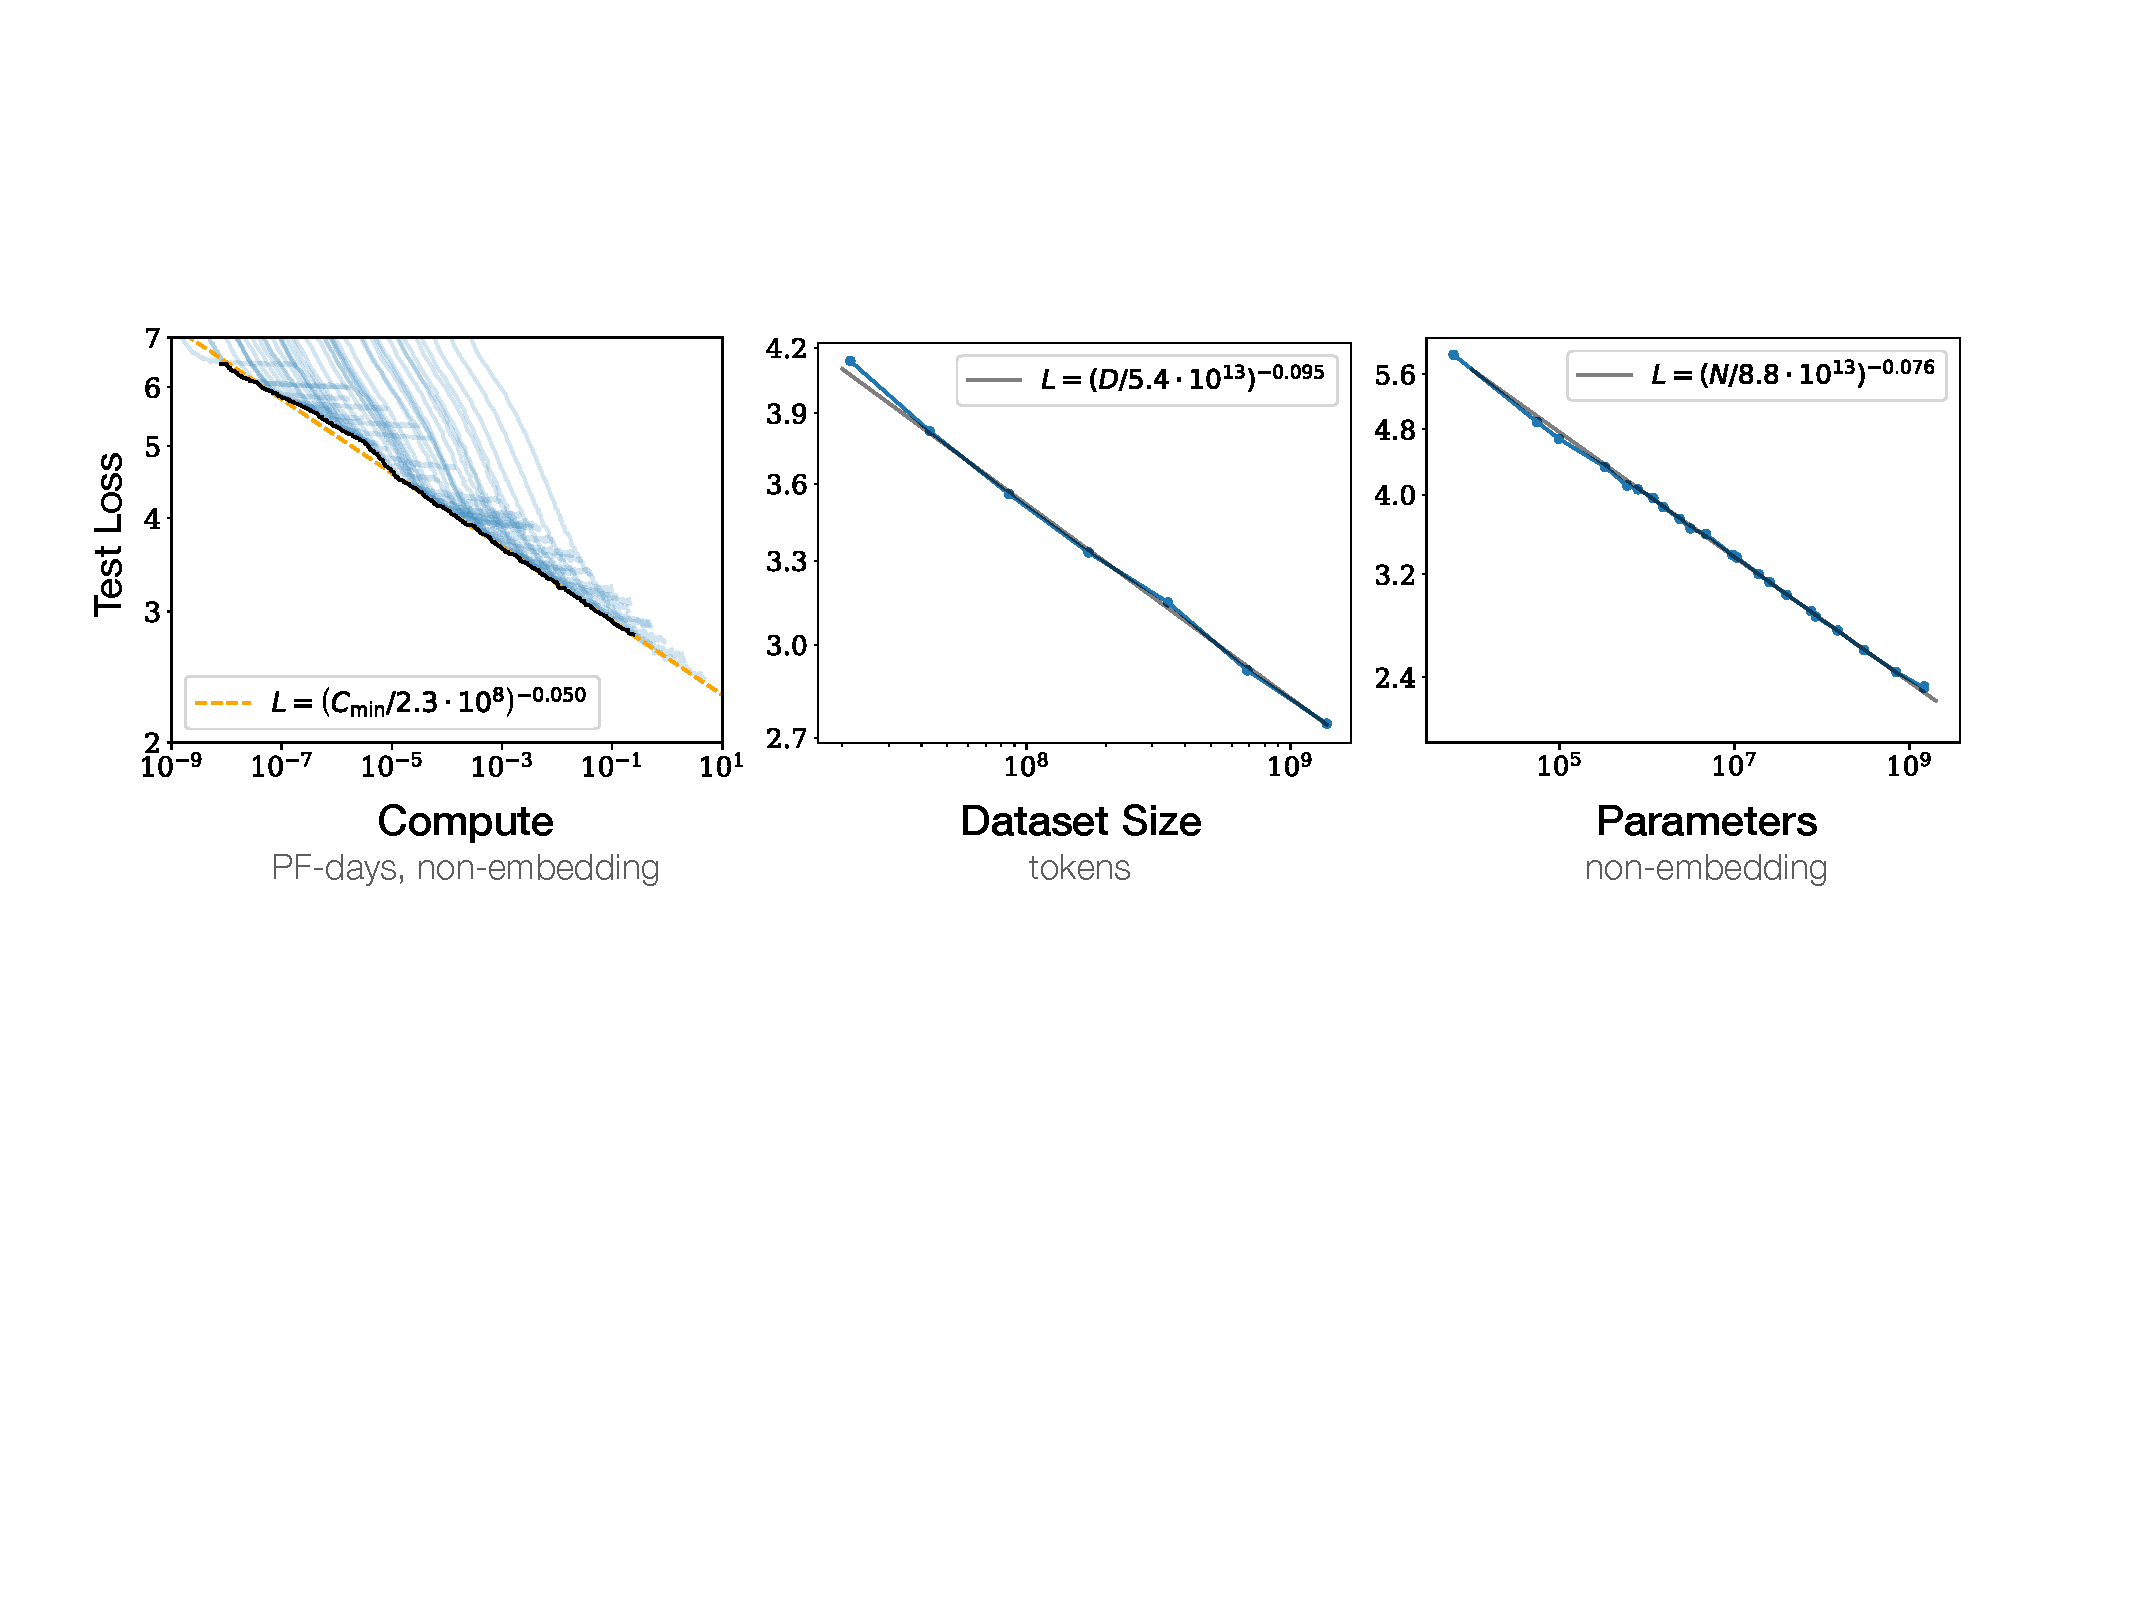
\includegraphics[scale=.5]{figures/SimplePowerLaws.pdf}
	\caption{Original scaling laws from \cite{kaplan2020scaling}.}
	\label{fig_scaling_laws_original_1}
\end{figure}


\begin{figure}[ht]
	\centering
	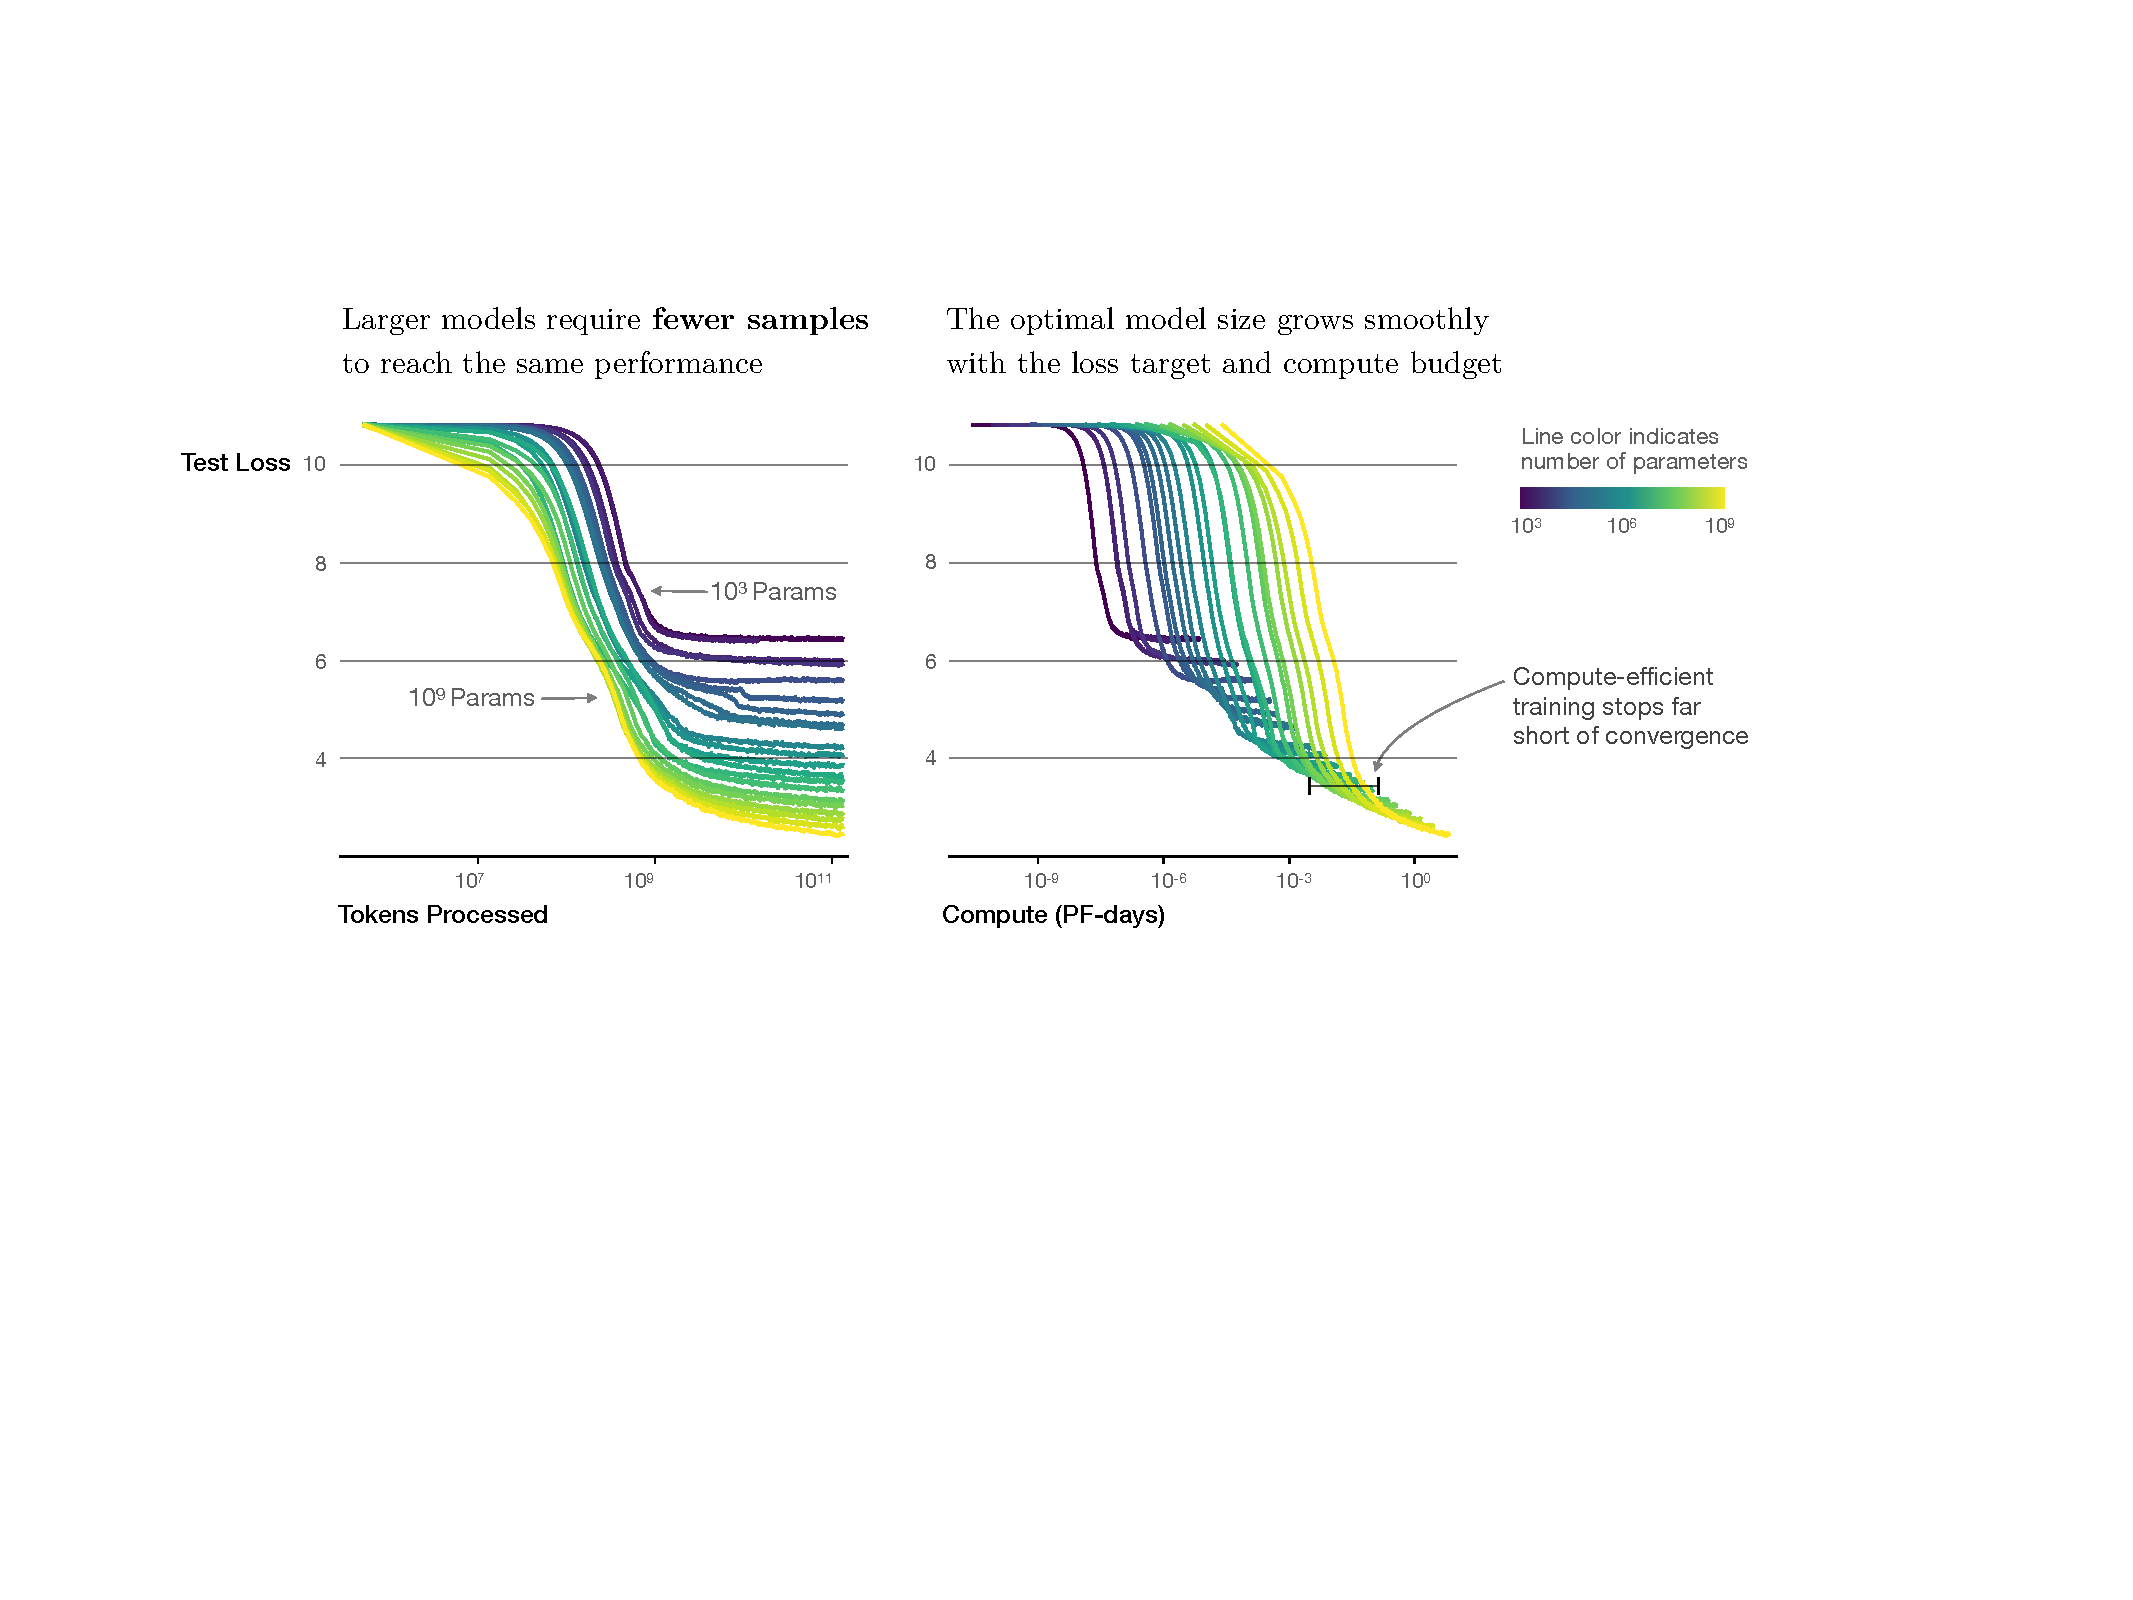
\includegraphics[scale=.5]{figures/EfficiencyIllustration.pdf}
	\caption{From \cite{kaplan2020scaling}. Larger models are much more sample-efficient (faster).}
	\label{fig_scaling_laws_original_2}
\end{figure}


\subsection{Chinchilla Scaling Laws}

As of Summer 2023, the Chinchilla scaling laws in \cite{hoffmann2022training} are the de facto best
scaling laws for guiding training. The central difference between \cite{hoffmann2022training} and
\cite{kaplan2020scaling} is that in the former they adjust their cosine learning-rate schedule to
reflect the amount of planned training, while in the latter they do not\footnote{The learning-rate
	schedule consist of a linear warm-up stage from a very small $ \eta  $ up to the largest value $ \eta _{ {\rm max} } $, after
	which the cosine bit kicks in: $ \eta (s)= \eta _{ {\rm min} } + \left ( \eta _{ {\rm max} } - \eta  _{ {\rm
				min} } \right ) \times \cos \left (\frac{ \pi s }{ 2 s _{ {\rm max} } }  \right) $ with $ s $ the
	step number. In Fig.~A1 of \cite{hoffmann2022training} they demonstrate that having the planned $ s
			_{ {\rm max} } $ duration of the scheduler be longer than the actual number of training steps is
	detrimental to training (they do not study the opposite regime), which is effectively what was done
	in \cite{kaplan2020scaling}. Probably the more important general point is again that the precise
	form of these scaling laws depend on details of fairly arbitrary training procedure choices, such as
	the choice of learning-rate scheduler.}.

Several different analyses are performed which all give very similar results. The outputs are the optimal values of $ N _{ {\rm params} }, N _{ {\rm tokens} } $ given a compute budget $ C $.
\begin{itemize}
	\item They fix various buckets of model sizes and train for varying lengths. In their resulting
	      loss-vs-FLOPs plot, they determine the model size which led to the best loss at each given FLOPs value, thereby generating
	      and optimal model size vs compute relation.
	\item They fix various buckets of FLOPs budget and train models of different sizes with that budget,
	      finding the optimal model size in each case. A line can then be fit to the optimal settings across
	      FLOPs budgets in both the parameter-compute and tokens-compute planes.
	\item  They perform a parametric fit to the loss\footnote{In \cite{hoffmann2022training} they model
		      the scaling of the test loss, while in \cite{kaplan2020scaling} they use the training loss.}:
	      \begin{align}
		      \Lcal (N _{ {\rm params} }, N _{ {\rm tokens} }) & =E + \frac{ A }{ N _{ {\rm  params} } ^{ \alpha  } }  + \frac{ B }{ N _{ {\rm tokens} } ^{ \beta  } } \label{eq_chinchilla} \ ,
	      \end{align}
	      fit over a large range of parameter and token choices. The best-fit values are:
	      \begin{align}
		      E & = 1.69 \ , \quad A = 406.4 \ , \quad B = 410.7 \ , \quad  \alpha = 0.34 \ , \quad \beta =0.28 \ .
	      \end{align}
	      Using $ C \approx 6 N _{ {\rm params}} N _{ {\rm tokens} } $, the above can be minimized at fixed compute
	      either for number of parameter or the size of the dataset.
\end{itemize}
In all cases, the findings are that at optimality  $ N _{ {\rm params} }  \sim N _{ {\rm tokens}
		}\sim C ^{ .5 } $: both the parameter and tokens budget should be scaled in equal measure.

